\documentclass[10pt,a4paper]{article}
\usepackage{hyperref}
\usepackage[latin1]{inputenc}
\usepackage{scrextend}
\usepackage[section]{placeins}
\usepackage[english]{babel}
\usepackage{listings}
\usepackage{amsmath}
\usepackage{amsfonts}
\usepackage{amssymb}
\usepackage{graphicx}
\usepackage{xcolor}
\usepackage{lstautogobble}
\usepackage[paper=portrait,pagesize]{typearea}
\author{Pascal Maczey \& Jan L�ffelsender - Team PJT}
\definecolor{groovyblue}{HTML}{0000A0}
\definecolor{groovygreen}{HTML}{008000}
\definecolor{darkgray}{rgb}{.4,.4,.4}

\lstdefinelanguage{Groovy}[]{Java}{
keywordstyle=\color{groovyblue}\bfseries,
stringstyle=\color{groovygreen}\ttfamily,
keywords=[3]{each, findAll, groupBy, collect, inject, eachWithIndex},
morekeywords={def, as, in, use},
moredelim=[is][\textcolor{darkgray}]{\%\%}{\%\%},
moredelim=[il][\textcolor{darkgray}]{§§},
autogobble=true
}
\title{Bakery project - OrderPorcessing- and DoughPreparation-Stage}
\begin{document}
	\maketitle
	\newpage
	\tableofcontents
	\newpage
	\section{How it works}
	
	
	\section{Design decisions}
	\subsection{OrderProcessing-Stage}
	\subsubsection{Splitting OrderProcessing and scheduling}
	The decision of splitting the OrderProcessing-Stage into to different agent is based on the idea of splitting functionality.
	\\
	The main idea of the OrderProcessing agent is to do all the communication with agents of different stages. That includes receiving a new order from a customer agent, making a proposal and so on.
	\\
	The scheduler agent should check if it's feasible to make an offer to the customer agent. That means the agent should check if all products are available and if it's possible to produce the products in time.
	\\
	These specifications has been changed a bit during development. To reduce communication between SchedulerAgent and OrderProcessing agent the OrderProcessing agent checks if any product is available. The reason for this decision is that a two way communication between Scheduler and OrderProcessing can be avoided. Next the SchedulerAgent sends the scheduled and accepted orders to the agents of the bakery. This way one message to the OrderProcessing agent is saved. But since the SchedulderAgent manages the Order Queue this decision is useful.
	
	\subsubsection{Reasons for behaviours in OrderProcessing}
	The TimeManager Behaviour controls if it is okay to start the new time step or if the agent should end. The reason to do this in an own behaviour was to loose the linkage of the time behaviour and the processing of messages and orders. Since it is (without additional synchronization) not possible to actively check if an order is coming at an specific timestep with the chosen implementation one timestep is lost every time an order is placed.
	\\
	The distributeFullOrder Behaviour propagates the whole order every time an order (call for proposal) arrives. This was specified in a task. The main reason is to notify the agents, that there might come a new scheduled order.
	\\
	The OfferRequestServer Behaviour handles all messages related with the Customer and the scheduler. The decision to combine this in only one Behaviour was, that a whole Order is processed at once.
	
	\subsubsection{Reasons for behaviours in SchedulerAgent}
	The reasons for the TimeManager Behaviour are the same as for the OrderProcessing agent.
	\\
	The isNewOrderChecker Behaviour checks for the distribution of a new full order which is distributed by OrderProcessing. If one is received the stepping forward in timesteps is blocked and the receiveOrder Behaviour is started.
	\\
	The receiveOrder Behaviour checks the schedule for all available products and only if for all available products the scheduling is possible it returns that scheduling is feasible. Last this behaviour add the order to schedule and queue if the proposal is accepted.
	
	\subsection{DoughPreparation-Stage}
		\subsubsection{Reason for representing preparing and kneading machines as objects}
		Kneading Machine and Preparing Machine are represented as an object based on the same class as
		The way we designed them there is not much functionality inside preparing machine and kneading machine
		Their only task it to update a counter and check whether a certain time threshold is reached
		\subsubsection{Reason for using the same class for preparing and kneading machines}
		For both objects the same class was used as both machines are very common - update a counter, store a state and update a boolean when finished.
		\subsubsection{Reason for making Dough Manager an agent}
		Most of the intelligent behaviour was moved to the dough manager. He contains kneading and preparing machines for one bakery. He manages orders which
		means moving one order from one state to next state, check whether current stage of dough preparing is finisehd, receiving orders from order processing agent
		and sending orders to proofer. The dough manager interacts with the environment (order processing agent and proofer) which means that he sends messages to the
		proofer and receives orders from order processing agent.
		\subsubsection{Reason for Behaviour in Dough Manager}
		The Dough Manager has the cyclic behaviour receive order. He pulls periodically for new messages. If there is a new message he processes it. This behaviour was chosen
		to make sure that all messages which are sent to dough manager are processed.
		\subsubsection{Reason for Proofer}
		The proofer was a design decision by the instructor to make sure that there is a well defined interface between the two stages dough preparation and baking stage.
		
	\section{Architectures}
	We used IntelliJ to generate the architecture. We present two versions because the full architecture\ref{fig:arch_full} isn't easily readable we generated a small\ref{fig:arch_small} one without internal classes, fields etc.
	\\
	The main usage of our architecture views is to show the composition of agents and objects and how they interact. Since the images are really big. They are included as images in the zip file.
	\newpage
	\KOMAoptions{paper=A3,paper=landscape,pagesize}
	\recalctypearea
	\begin{figure}[hbt!]
		\hspace*{-6cm}
		\centering
		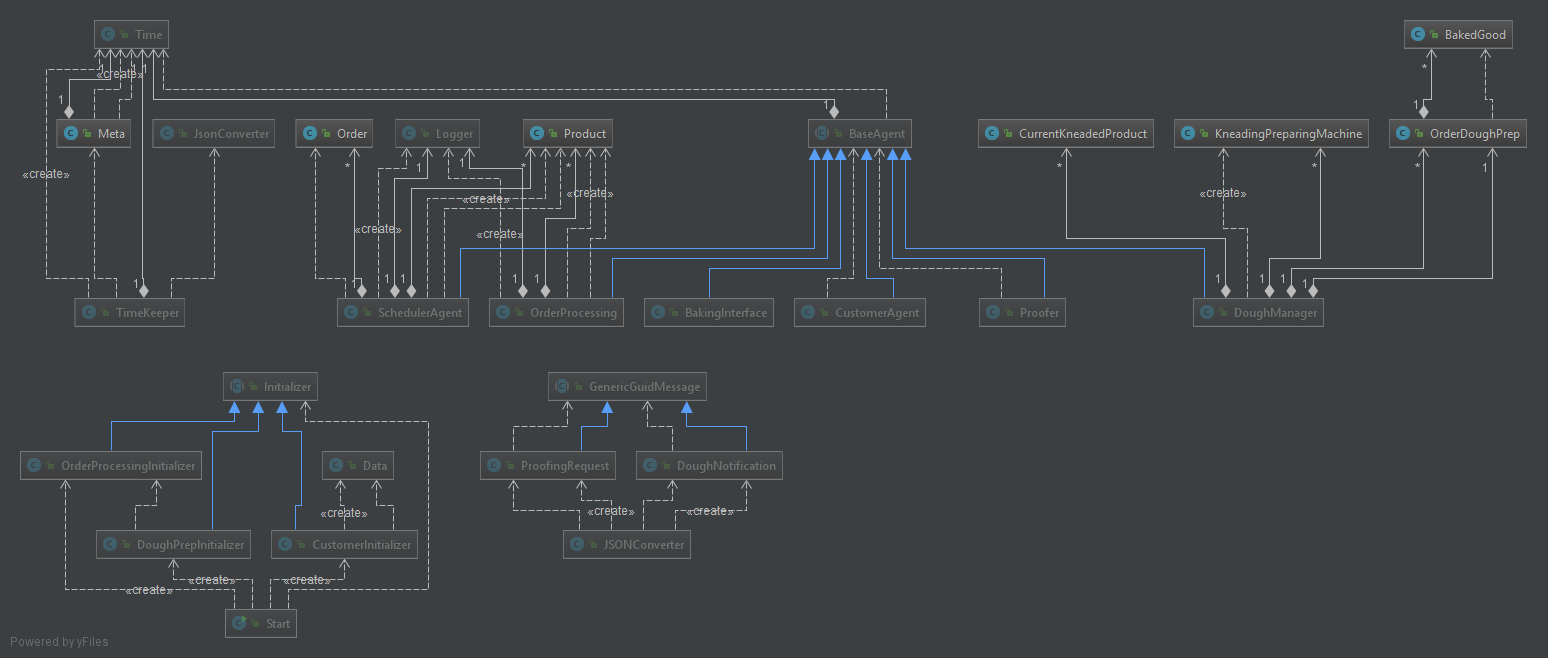
\includegraphics[width=0.9\paperwidth]{Architecture_small.png}
		\caption{This image shows the reduced architecture.}
		\label{fig:arch_small}
	\end{figure}
	\newpage
	\begin{figure}[hbt!]
		\hspace*{-6cm}
		\centering
		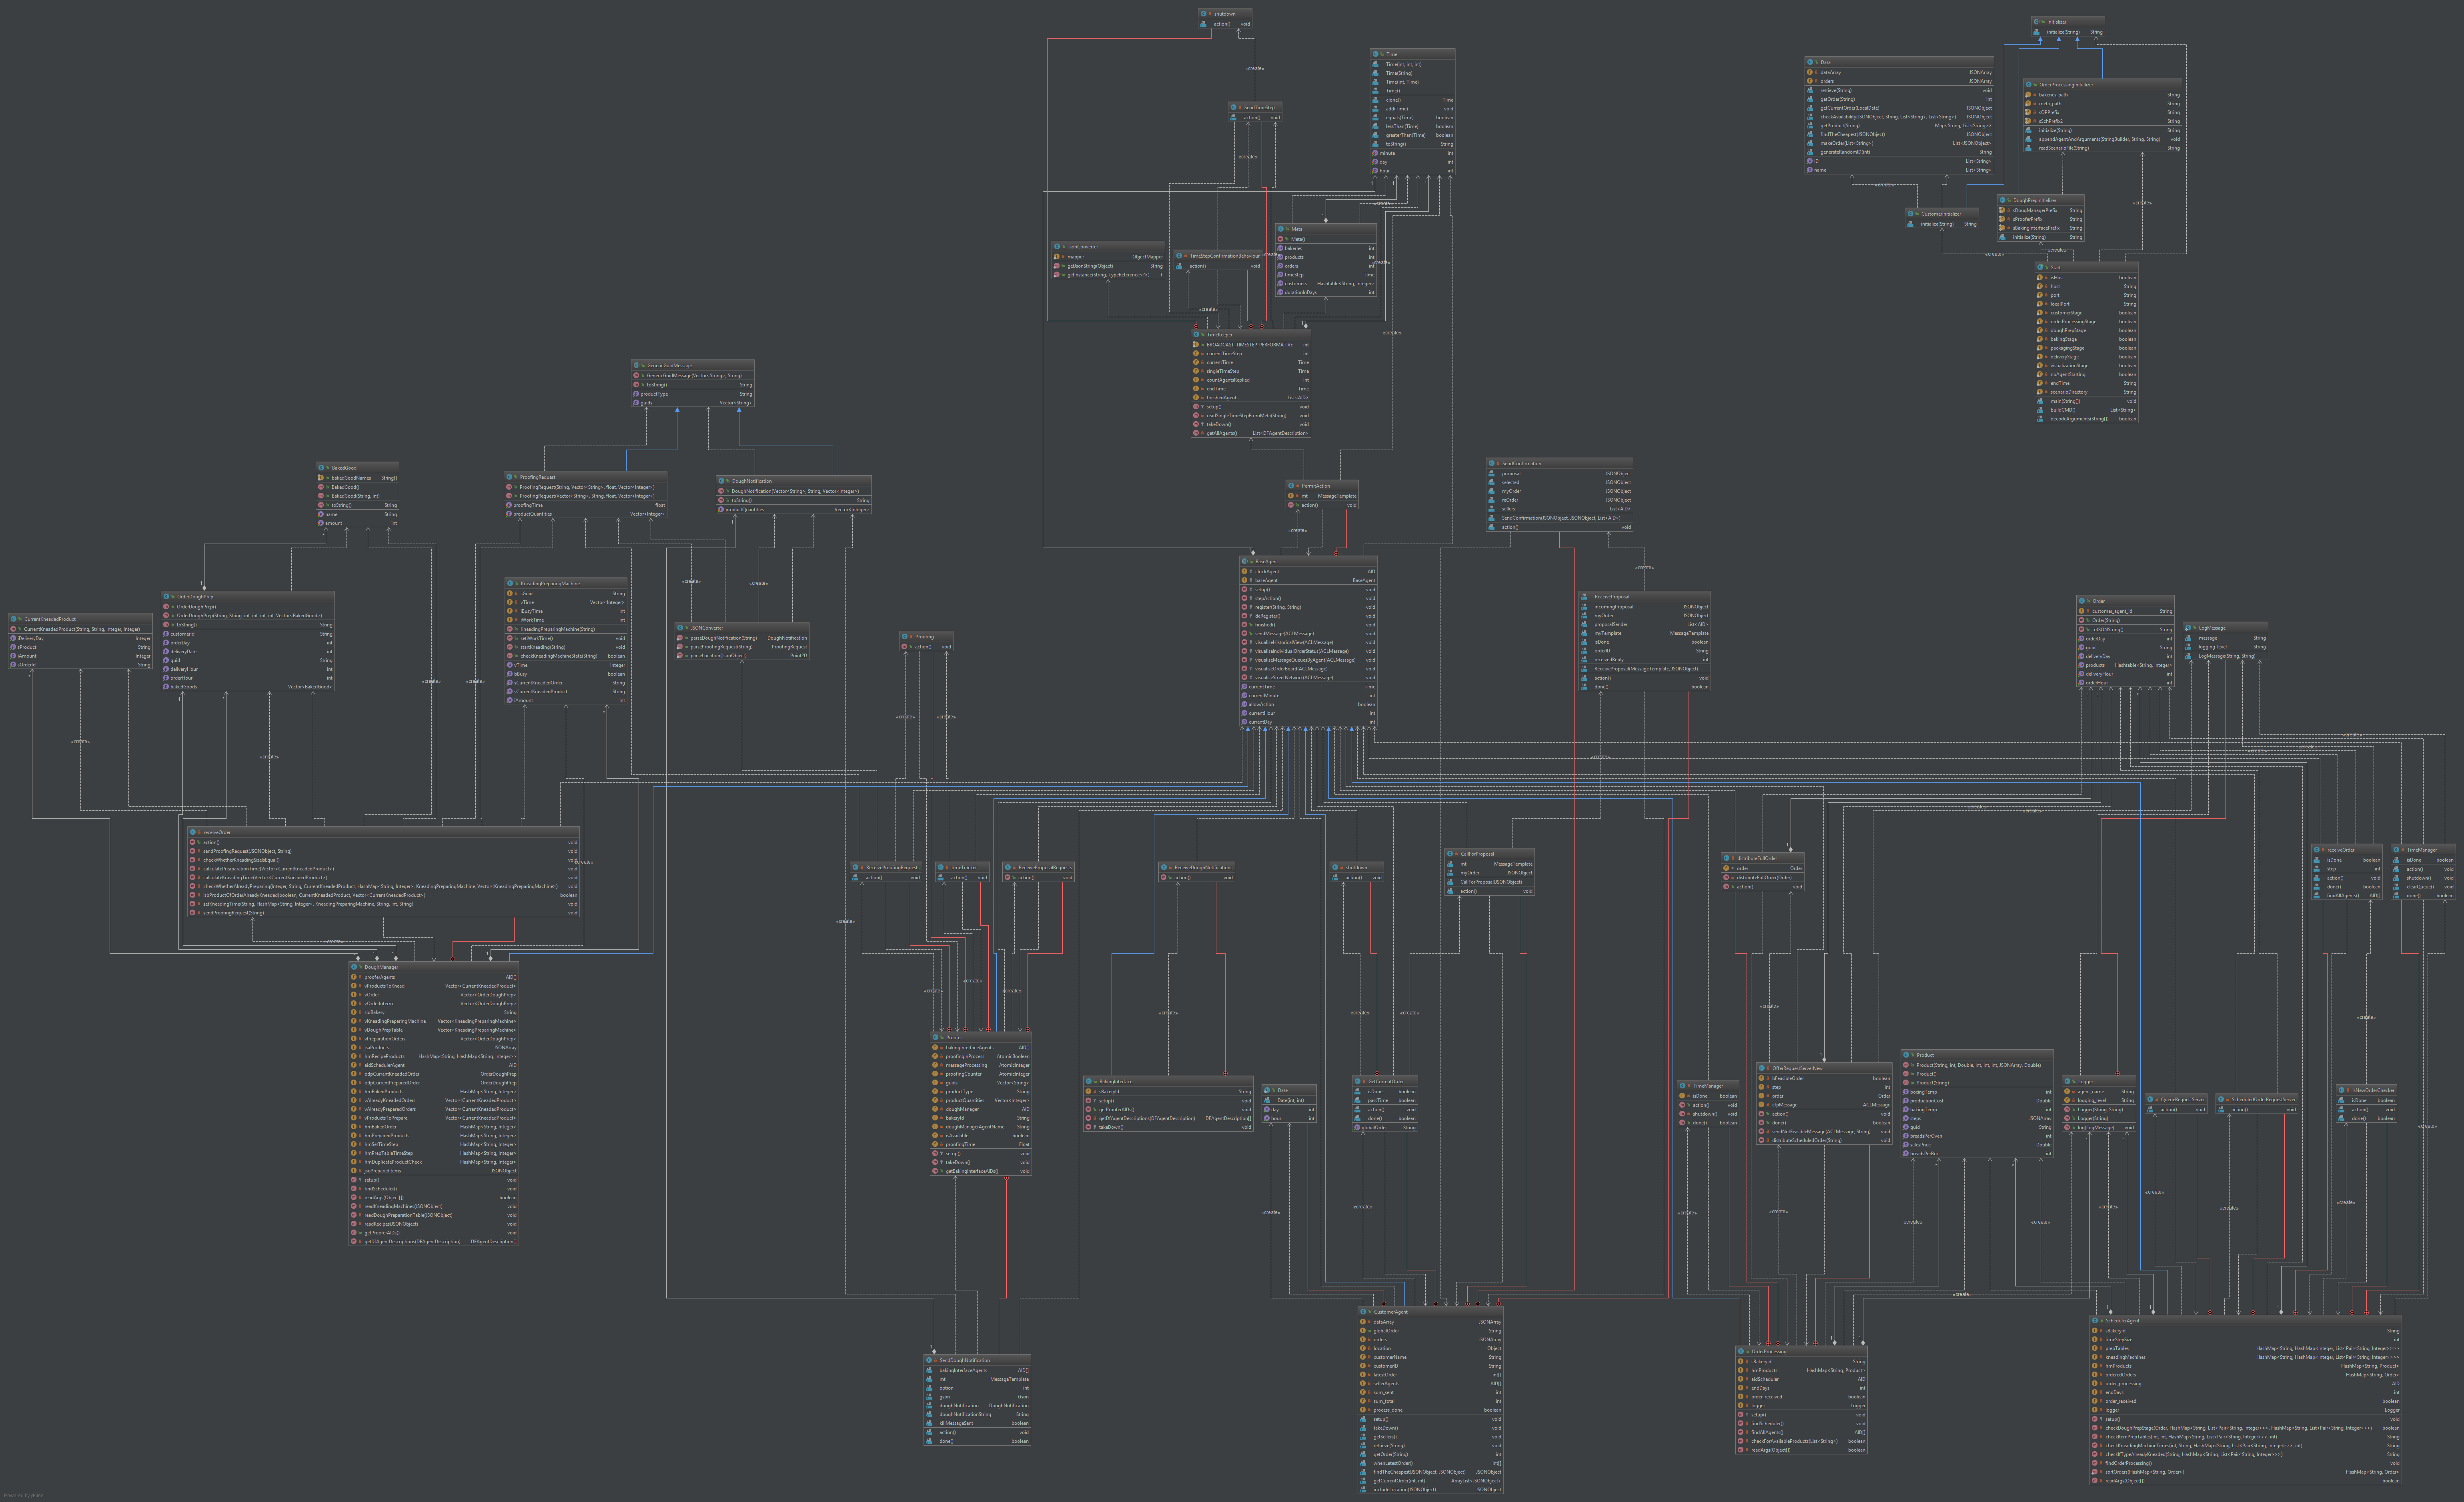
\includegraphics[width=0.9\paperwidth]{Architecture_full.png}
		\caption{This image shows the full architecture.}
		\label{fig:arch_full}
		
	\end{figure}

	\newpage
	\FloatBarrier
	\KOMAoptions{paper=A4,paper=portrait,pagesize}
	\recalctypearea
	\section{Messages}
	In the following table you can see each message receive or send by any of our agents.
	\begin{itemize}
		\item Receive Order from client:
		\begin{itemize}
			\item Type: CFP
			\item From: CustomerAgent
			\item To: OrderProcessing
			\item ConversationId: {orderId}
			\item Content: JSONObject as String -\textgreater Order
		\end{itemize}
		\item Receive accepted proposal:
		\begin{itemize}
			\item Type: ACCEPT\_PROPOSAL
			\item From: CustomerAgent
			\item To: OrderProcessing
			\item ConversationId: {orderId}
			\item Content: JSONObject as String -\textgreater Full Order but only containing products available at specified bakery
		\end{itemize}
		\item Receive reject proposal:
		\begin{itemize}
			\item Type: REJECT\_PROPOSAL
			\item From: CustomerAgent
			\item To: OrderProcessing
			\item ConversationId: {orderId}
			\item Content: String -\textgreater \glqq rejected\grqq
		\end{itemize}
		\item Confirm Schedule:
		\begin{itemize}
			\item Type: CONFIRM
			\item From: SchedulerAgent
			\item To: OrderProcessing
			\item ConversationId: -
			\item Content: String -\textgreater \glqq Scheduling possible\grqq
		\end{itemize}
		\item Disconfirm Schedule:
		\begin{itemize}
			\item Type: DISCONFIRM
			\item From: SchedulerAgent
			\item To: OrderProcessing
			\item ConversationId: -
			\item Content: String -\textgreater \glqq Scheduling impossible\grqq
		\end{itemize}
		\item Proposal to Client:
		\begin{itemize}
			\item Type: PROPOSAL
			\item From: OrderProcessing
			\item To: CustomerAgent
			\item ConversationId: {orderId}
			\item Content: JSONObject as String -\textgreater List of available products with prices (amount of product times sales\_price for product)
		\end{itemize}
		\item DistributeReceivedOrder:
		\begin{itemize}
			\item Type: INFORM
			\item From: OrderProcessing
			\item To: all agents of same bakery
			\item ConversationId: -
			\item Content: JSONObject as String -\textgreater Order
		\end{itemize}
		\item Refusal to Customer
		\begin{itemize}
			\item Type: REFUSE
			\item From: OrderProcessing
			\item To: CustomerAgent
			\item ConversationId: -
			\item Content: String -\textgreater reason for refusal (no needed product available or not enough time to produce order)
		\end{itemize}
		\item Check Scheduler
		\begin{itemize}
			\item Type: REQUEST
			\item From: OrderProcessing
			\item To: SchedulerAgent
			\item ConversationId: -
			\item Content: JSONObject as String -\textgreater order with only available products
		\end{itemize}
		\item Send acceptes Order to Scheduler
		\begin{itemize}
			\item Type: PROPAGATE
			\item From: OrderProcessing
			\item To: SchedulerAgent
			\item ConversationId: -
			\item Content: JSONObject as String -\textgreater Order containing only Products that should be produced by this bakery
		\end{itemize}
		\item Propagate accepted Orders:
		\begin{itemize}
			\item Type: PROPAGATE
			\item From: OrderProcessing
			\item To: SchedulerAgent
			\item ConversationId: -
			\item Content: JSONObject as String -\textgreater Order containing only Products that should be produced by this bakery
		\end{itemize}
		\item Check Scheduler:
		\begin{itemize}
			\item Type: REQUEST
			\item From: OrderProcessing
			\item To: SchedulerAgent
			\item ConversationId: -
			\item Content: JSONObject as String -\textgreater order with only available products
		\end{itemize}
		\item Get Queue Position:
		\begin{itemize}
			\item Type: REQUEST
			\item From: AnyAgent
			\item To: SchedulerAgent
			\item ConversationId: \glqq queue request\grqq
			\item Content: String -\textgreater {orderId}
		\end{itemize}
		\item Confirm Schedule:
		\begin{itemize}
			\item Type: CONFIRM
			\item From: SchedulerAgent
			\item To: OrderProcessing
			\item ConversationId: -
			\item Content: String -\textgreater \glqq Scheduling possible\grqq
		\end{itemize}
		\item Disconfirm Schedule:
		\begin{itemize}
			\item Type: DISCONFIRM
			\item From: SchedulerAgent
			\item To: OrderProcessing
			\item ConversationId: -
			\item Content: String -\textgreater \glqq Scheduling impossible!\grqq
		\end{itemize}
		\item Propagate acceptedOrders:
		\begin{itemize}
			\item Type: PROPAGATE
			\item From: SchedulerAgent
			\item To: All receiving Agents of same bakery
			\item ConversationId: -
			\item Content: JSONArray as String -\textgreater sorted List of accepted Orders
		\end{itemize}
		\item Queue request reply:
		\begin{itemize}
			\item Type: INFORM
			\item From: Scheduler Agent
			\item To: Any agent
			\item ConversationId: \glqq queue request\grqq
			\item Content: String -\textgreater Order position if order in queue else -1
		\end{itemize}
		\item ScheduledOrders reply
		\begin{itemize}
			\item Type: INFORM
			\item From: SchedulerAgent
			\item To: Any Agent
			\item ConversationId: -
			\item Content: JSONArray as String -\textgreater All scheduled orders
		\end{itemize}
		\item Sends proofing request to proofer:
		\begin{itemize}
			\item Type: ACCEPT\_PROPOSAL
			\item From: DoughManager of bakery
			\item To: Proofer
			\item ConversationId: -
			\item Content: JSONObject as String -\textgreater Order products
		\end{itemize}
		\item Receive order vector from SchedulerAgent:
		\begin{itemize}
			\item Type: PROPAGATE
			\item From: SchedulerAgent
			\item To: DoughManager
			\item ConversationId: -
			\item Content: JSONArray as String -\textgreater Order
		\end{itemize}
	\end{itemize}
	Content of Message \glqq Sends proofing request to proofer\grqq and \glqq Receive order vector from SchedulerAgent\grqq.
	\begin{lstlisting}[frame=single]
Receive order vector from SchedulerAgent content:
[
  {
    "customerId": String,
    "guid": String,
    "deliveryDate": JSONObject,
    "orderDate": JSONObject,
    "products": JSONObject
  },
  .
  .
]

Exampe Content:
[
  {
    "customerId":"customer-014",
    "guid":"order-583","deliveryDate":{"hour":17,"day":2},
    "orderDate":{"hour":2,"day":1},
    "products":{"Donut":7,"Bagel":7,"Bread":3}
  },
  {
    "customerId":"customer-001",
    "guid":"order-001",
    "deliveryDate":{"hour":18,"day":2},
    "orderDate":{"hour":4,"day":1},
    "products":{"Donut":7,"Bagel":6,"Berliner":2,"Muffin":2,
                                                 "Bread":10}
  },
  .
  .
]

Sends proofing request to proofer:
{
  "proofingTime": Integer,
  "productQuantities": Vector<Integer>,
  "guids": String,
  "productType": String
}



Example Content:
{
  "proofingTime":12.0,
  "productQuantities":[1],
  "guids":["order-583"],
  "productType":"Bread"
}
	\end{lstlisting}
	\section{Agents}
	Agents per pakery:
	\begin{enumerate}
		\item [-] Scheduler $\rightarrow$ Is needed to schedule orders. It checks whether the order can be processed - so is there enough time to prepare the order
		under given circumstances?
		\item [-] OrderProcessing $\rightarrow$ The Order Procesing agent receives an order from the client, distributes the order to all agents, talks to the scheduler
		to verify whether order is feasible and gives the customer a hint whether its order can be processed or not.
		\item [-] DoughManager $\rightarrow$ He manages the kneading machines and preparation tables for one bakery. He ensures that its kneading machines and preparation
		tables are synchron with the time keeper, checks whether current kneaded and prepared products are finished and sends kneaded and prepared orders to proofer.
		\item [-] Proofer $\rightarrow$ The proofer proofs the orders and sends them to the bakery.
	\end{enumerate}
	\section{Objects}
	Objects :
	\begin{enumerate}
		\item [-] BakedGood $\rightarrow$ Name of product and the amount of it for one order within DoughPreparationStage.
		\item [-] CurrentProcessedProduct $\rightarrow$ An object which describes the current kneaded product. In other
		context it is used to describe the current prepared product. Moreover it is used to remeber already kneaded
		and prepared products.
		\item [-] KneadingPreparingMachine $\rightarrow$ Describes kneading and preparing machines. It stores the current
		kneaded / prepared order , the progress of preparing / kneading and it checks whether the preparation has finished
		\item [-] Order $\rightarrow$ An object for Scheduler and OrderProcessing Agent. It stores information as customer
		agent id, order day, order hour, delivery day and delivery hour.
		\item [-] OrderDoughPrep $\rightarrow$ An object for storing received orders from Scheduler.
		\item [-] Product $\rightarrow$ An object which stores information on the product (preparation time,
		salesPrice, boxingTemp, guid)
	\end{enumerate}
	\section{How to run it}
	The Start.java is configured in order to run this project easily.
	In order to run our two stages and the customer Stage (which is copied from the upstream) just use:

	\begin{lstlisting}[language=Groovy,caption = Gradle run,frame=single, label={gradlerun} ]
	gradle run
	\end{lstlisting}

	\noindent It will automatically get the dependencies and start JADE with the configured agents.
	In case you want to clean you workspace run

	\begin{lstlisting}[language=Groovy,caption = Gradle clean,frame=single, label={gradleclean} ]
	gradle clean
	\end{lstlisting}
	If you want to see all possible options how the project can be run use:
	\begin{lstlisting}[language=Groovy,caption = Gradle run args,frame=single, label={gradlerunargs} ]
	gradle run --args='-h'
	\end{lstlisting}
\end{document}